\section{Introduction}

A Large Ion Collider Experiment (ALICE) has been proposed and built to study
the properties of the Quark-Gluon Plasma in hadronic collisions at the Large
Hadron Collider at CERN~\cite{Aamodt:2008zz}.

\begin{itemize}
\item overview of the detector
  (status as of end of Run 2)
\item barrel tracking
\item detectors for particle identification
\item calorimetry
\item forward physics
\item triggering
\end{itemize}

\begin{figure}
\centering
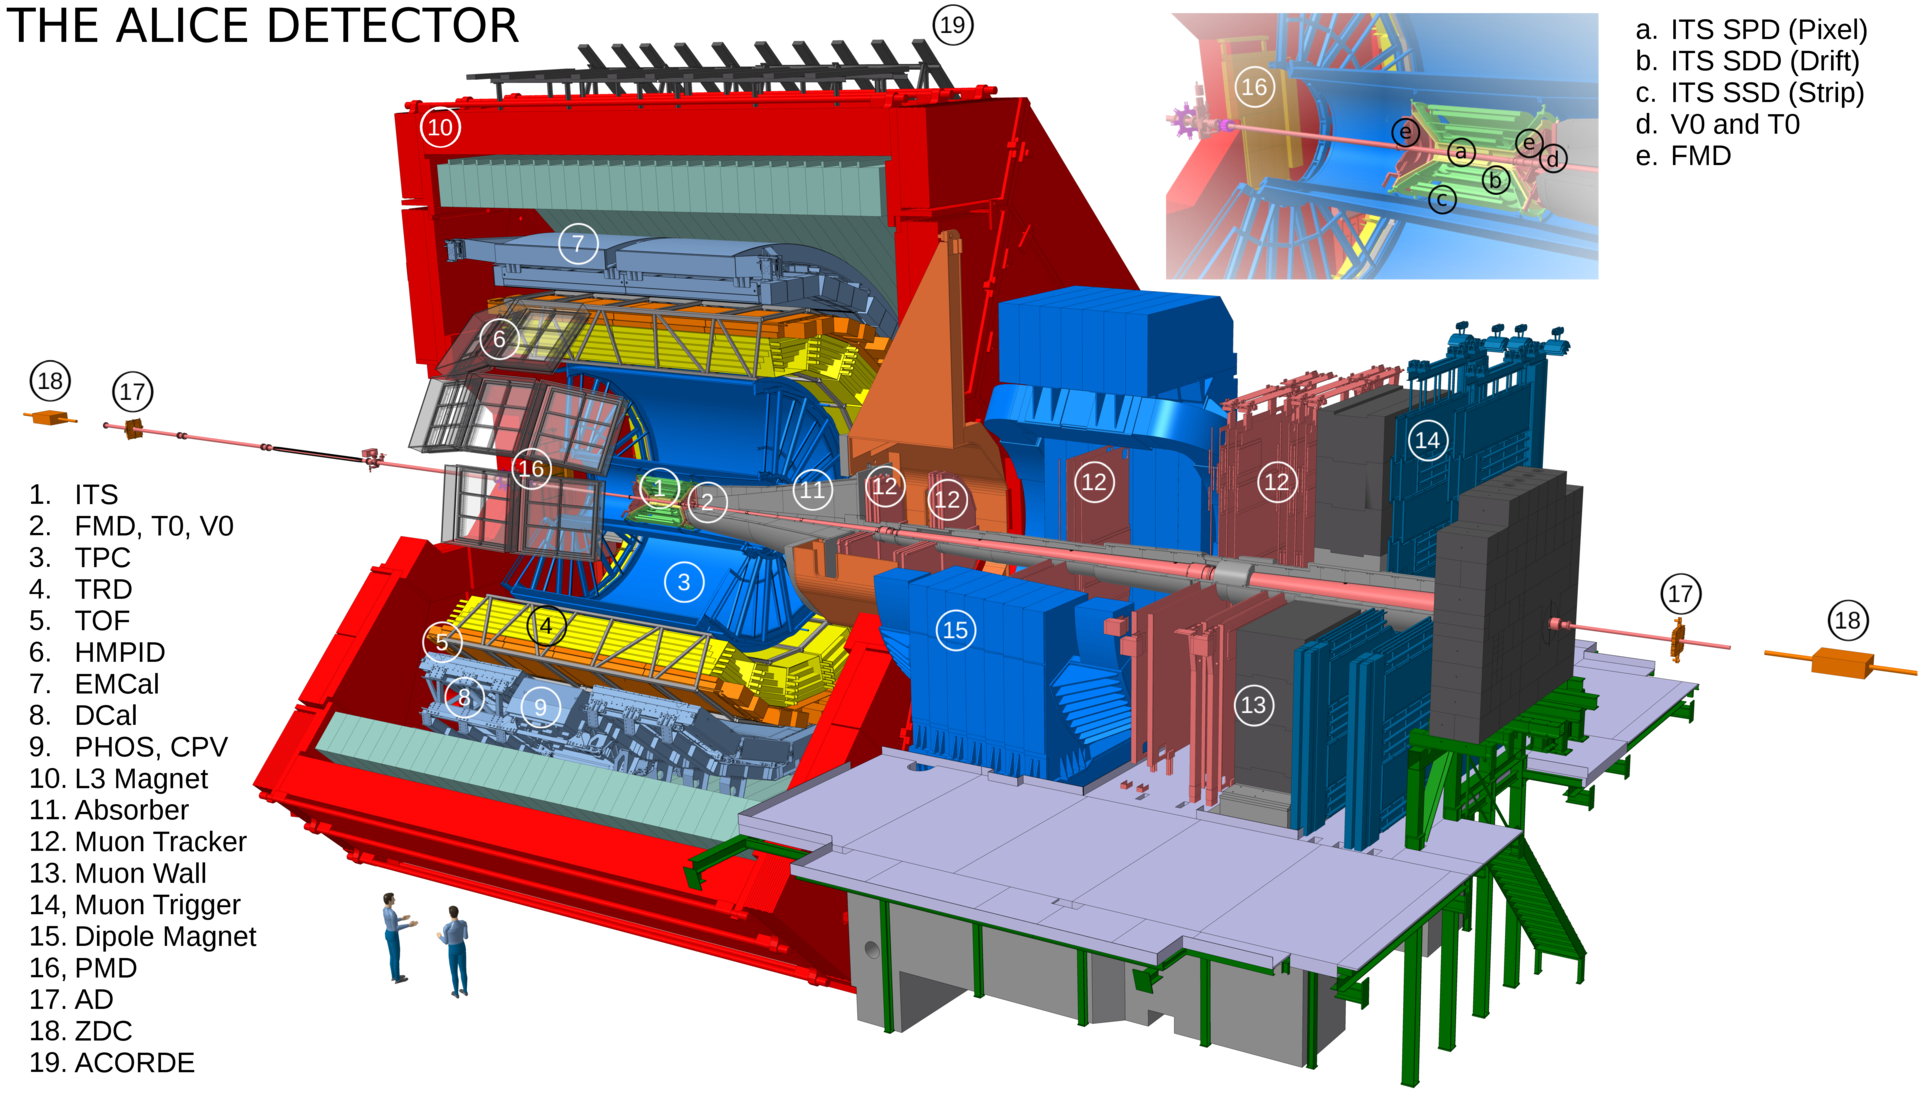
\includegraphics[width=.7\textwidth]{intro/2017-May-11-ALICE_RUN2_labels_HD}
\caption{Overview Run 2}
\label{fig:alice_run2}
\end{figure}

\subsection{Run1/2 performance highlights (examples)}

cite performance paper~\cite{Abelev:2014ffa}, possibly also detector papers

discuss performance
\begin{itemize}
\item particle identification
\item secondary vertex resolution
\item data sets (rate/integrated luminosity)
\end{itemize}
